\documentclass[12pt,letterpaper]{article}

\usepackage[utf8]{inputenc}
\usepackage[T1]{fontenc}
\usepackage[spanish]{babel}
\decimalpoint

\usepackage{amsmath, amsfonts, amssymb, amsthm}
\usepackage{graphicx}
\usepackage{subfigure}
\usepackage{multicol}
\usepackage{tcolorbox}
\usepackage{pgf, tikz}
\usepackage{mathrsfs}
\usepackage{fancyhdr}
\usepackage{caption}
\usepackage{cancel}
\usepackage{listingsutf8}
\usepackage{color}
\usepackage{algpseudocode}
\usepackage{hyperref}
\usepackage[paper=letterpaper, right=2.5cm, left=2.5cm, top=3cm, bottom=2.2cm]{geometry}

\setlength{\parindent}{0pt}
\setlength{\parskip}{0em}

% Librerías de TikZ
\usetikzlibrary{arrows}
\usetikzlibrary{babel}

% Comandos personalizados
\newcommand{\N}{\mathbb{N}}
\newcommand{\C}{\mathbb{C}}
\newcommand{\R}{\mathbb{R}}
\newcommand{\Q}{\mathbb{Q}}
\newcommand{\Z}{\mathbb{Z}}

\newcommand{\myfloor}[1]{\left\lfloor #1 \right\rfloor}
\newcommand{\myceil}[1]{\left\lceil #1 \right\rceil}
\newcommand{\mypar}[1]{\left( #1 \right)}
\newcommand{\mycor}[1]{\left[ #1 \right]}
\newcommand{\ndiv}{\hspace{-4pt}\not|\hspace{2pt}}

% Teoremas
\theoremstyle{definition}
\newtheorem{defi}{Definición}[section]
\newtheorem{ejemplo}{Ejemplo}[section]
\newtheorem{problem}{Problema}[section]
\newtheorem{ejer}{Ejercicio}[section]

\theoremstyle{plain}
\newtheorem{teo}{Teorema}[section]
\newtheorem{colo}{Corolario}[section]
\newtheorem{lema}{Lema}[section]
\newtheorem{conj}{Conjetura}[section]
\newtheorem{propo}{Proposición}[section]

\theoremstyle{remark}
\newtheorem{obser}{Observación}[section]

% Teoremas coloreados con tcolorbox
\tcbuselibrary{theorems}
\newtcbtheorem[number within=section]{mytheo}{Teorema}%
{colback=green!5,colframe=green!35!black,fonttitle=\bfseries}{th}

\newtcbtheorem[number within=section]{mydefi}{Definición}%
{colback=red!5,colframe=red!35!black,fonttitle=\bfseries}{th}

% Cálculo de formatos numéricos
\usepackage{expl3, xparse}
\ExplSyntaxOn
\DeclareDocumentCommand { \myformat }{m}
  { \fp_to_decimal:n { round((#1),9) } }
\ExplSyntaxOff

% Configuración de código MATLAB
\definecolor{mygreen}{RGB}{28,172,0}
\definecolor{mylilas}{RGB}{170,55,241}

\lstset{
    language=Matlab,
    breaklines=true,
    morekeywords={matlab2tikz},
    keywordstyle=\color{blue},
    morekeywords=[2]{1}, keywordstyle=[2]{\color{black}},
    identifierstyle=\color{black},
    stringstyle=\color{mylilas},
    commentstyle=\color{mygreen},
    showstringspaces=false,
    numbers=left,
    numberstyle={\tiny \color{black}},
    numbersep=9pt,
    emph=[1]{for,end,break},
    emphstyle=[1]\color{red},
    literate=
         {á}{{\'a}}1 {í}{{\'i}}1 {é}{{\'e}}1 {ú}{{\'u}}1 {ó}{{\'o}}1
         {Á}{{\'A}}1 {Í}{{\'I}}1 {É}{{\'E}}1 {Ú}{{\'U}}1 {Ó}{{\'O}}1
}

% Información del documento
\author{Ricardo Largaespada}
\title{\textbf{Métodos Numéricos | Laboratorio 3}}
\date{27 de marzo de 2025}

\usepackage{eso-pic}

\begin{document}

\maketitle

\AddToShipoutPictureBG{
\includegraphics[width=\paperwidth,height=\paperheight]{fondo.pdf}}

\section{Introducción}
Durante la clase anterior, trabajamos con métodos cerrados para encontrar raíces de ecuaciones. En dichos métodos, la raíz se encuentra dentro de un intervalo predeterminado, delimitado por un valor inferior y uno superior. La aplicación repetida de estos métodos genera aproximaciones cada vez más cercanas a la raíz. Se dice que estos métodos son {\it convergentes} porque se acercan progresivamente a la raíz a medida que se avanza en el cálculo.\\

En esta sesión, estudiaremos los llamados métodos abiertos. A diferencia de los métodos cerrados, estos se basan en fórmulas que requieren únicamente de un valor inicial $x$ (o un par de valores), pero que no necesariamente encierran la raíz dentro de un intervalo. Como resultado, estos métodos pueden —en algunos casos— alejarse de la raíz verdadera a medida que se itera. Sin embargo, cuando convergen, suelen hacerlo mucho más rápido que los métodos cerrados.

Comenzaremos el análisis de los métodos abiertos con una versión simple que es útil para ilustrar su funcionamiento general y también para introducir formalmente el concepto de convergencia.

\section{Iteración por Punto Fijo}

El método de iteración por punto fijo es una técnica sencilla y poderosa para aproximar raíces de ecuaciones no lineales. Es un método abierto que requiere una buena elección del valor inicial para asegurar su convergencia.

\subsection*{Idea del método}

Partimos de una ecuación de la forma:
\(f(x) = 0\) y la reescribimos como:
\(x = g(x).\)

Esta nueva forma se denomina {\bf forma iterativa}, ya que nos permite generar una secuencia de valores:
\[
x_{i+1} = g(x_i)
\]

A partir de un valor inicial $x_0$, se genera un nuevo valor usando $g(x_0)$, luego $g(x_1)$, y así sucesivamente. Este proceso continúa hasta que el valor calculado cambie muy poco con respecto al anterior (es decir, hasta que el error relativo aproximado sea menor que un valor de tolerancia predefinido).

\subsection*{Criterio de convergencia}

El método de punto fijo converge si en la vecindad de la raíz se cumple:
\[
|g'(x)| < 1
\]
Esto significa que la función iterativa $g(x)$ debe tener una pendiente suficientemente pequeña cerca de la solución para asegurar que las sucesivas aproximaciones se acerquen a la raíz.

\subsection*{Cálculo del error}

El error relativo aproximado en cada iteración puede estimarse con:
\[
\varepsilon_a = \left| \frac{x_{i+1} - x_i}{x_{i+1}} \right| \cdot 100\%
\]

\subsection*{Ventajas y desventajas}

\begin{itemize}
    \item {\bf Ventajas:} Es fácil de implementar y no requiere derivadas.
    \item {\bf Desventajas:} No siempre converge. La elección de la función $g(x)$ es clave.
\end{itemize}

\subsection*{Pseudocódigo del método}

\begin{algorithmic}[1]
\Function{PuntoFijo}{x0, es, imax}
    \State xr $\gets$ x0
    \State iter $\gets$ 0
    \Repeat
        \State xrold $\gets$ xr
        \State xr $\gets$ g(xrold)
        \State iter $\gets$ iter + 1
        \If{xr $\neq$ 0}
            \State ea $\gets \left| \dfrac{xr - xrold}{xr} \right| \cdot 100$
        \EndIf
    \Until{ea < es {\bf or} iter $\geq$ imax}
    \State \Return xr
\EndFunction
\end{algorithmic}

\subsection*{Observación importante}

No toda reescritura de $f(x) = 0$ como $x = g(x)$ asegura convergencia. Por eso, antes de aplicar el método es recomendable verificar gráficamente o analíticamente si la función $g(x)$ cumple con el criterio de convergencia en el intervalo de interés.

\section{Método de Newton-Raphson}

El método de Newton-Raphson es uno de los métodos abiertos más populares para encontrar raíces de funciones no lineales. Su principal ventaja es que, si se aplica correctamente y con una buena estimación inicial, puede converger de manera muy rápida a la solución.

El único inconveniente es que requiere conocer no solo la función $f(x)$, sino también su derivada $f'(x)$. Por esta razón, es aplicable únicamente cuando la derivada puede ser calculada con facilidad.

\subsection*{Derivación de la fórmula}

La fórmula del método de Newton-Raphson se puede obtener a partir de la serie de Taylor de $f(x)$ centrada en el punto $x_i$:
\begin{align}
f(x_{i+1}) = f(x_i) + f'(x_i)(x_{i+1}-x_i) + O((x_{i+1}-x_i)^2) \label{eq:6}
\end{align}

Si asumimos que $x_{i+1}$ es una raíz de $f(x)$, entonces $f(x_{i+1}) = 0$. Sustituyendo en la ecuación anterior y descartando el término de orden superior, se obtiene:
\begin{align}
0 = f(x_i) + f'(x_i)(x_{i+1}-x_i) \label{eq:7}
\end{align}

Despejando $x_{i+1}$ se llega a la forma iterativa:
\begin{align}
x_{i+1} = x_i - \frac{f(x_i)}{f'(x_i)} \label{eq:8}
\end{align}

Esta fórmula se aplica de forma repetida, generando nuevas aproximaciones de la raíz en cada paso.

\subsection*{Convergencia del método}

Si $x$ es la raíz exacta, el error en la iteración $i$ se define como $E_i = x - x_i$. Puede demostrarse que el error en la siguiente iteración está dado por:
\[
E_{i+1} = - \frac{f''(x_i)}{2f'(x_i)} E_i^2
\]

Este resultado implica que el método tiene {\bf convergencia cuadrática}: si $x_i$ está suficientemente cerca de la raíz, el número de cifras significativas se duplica aproximadamente en cada iteración.

\begin{figure}[h!]
\centering
\subfigure[Converge]{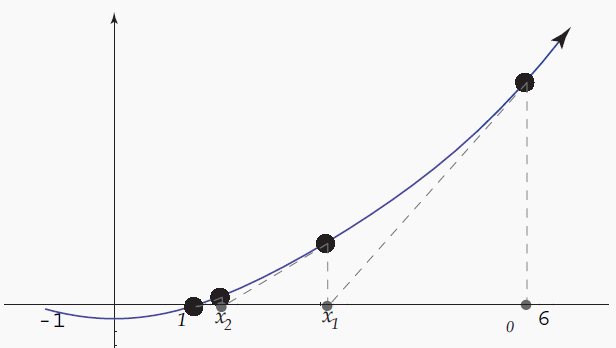
\includegraphics[scale=0.3]{images/Clase3-f2-a.PNG}}
\subfigure[Diverge]{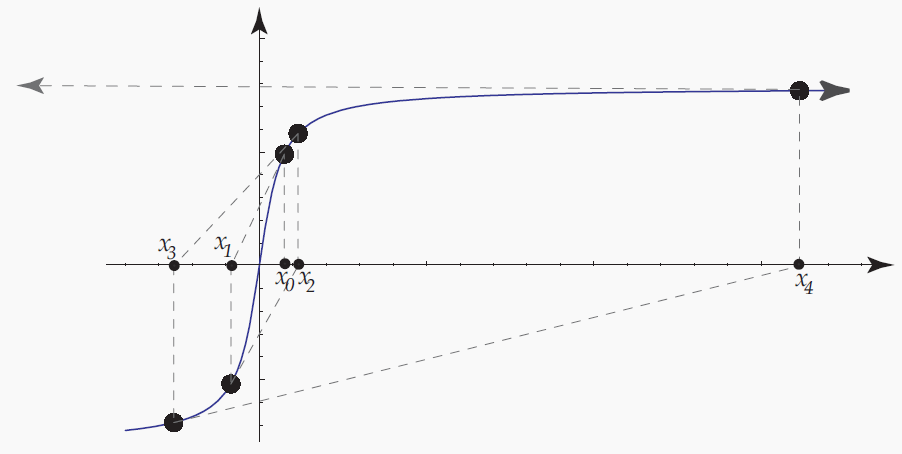
\includegraphics[scale=0.25]{images/Clase3-f2-b.PNG}}
\subfigure[Ciclo]{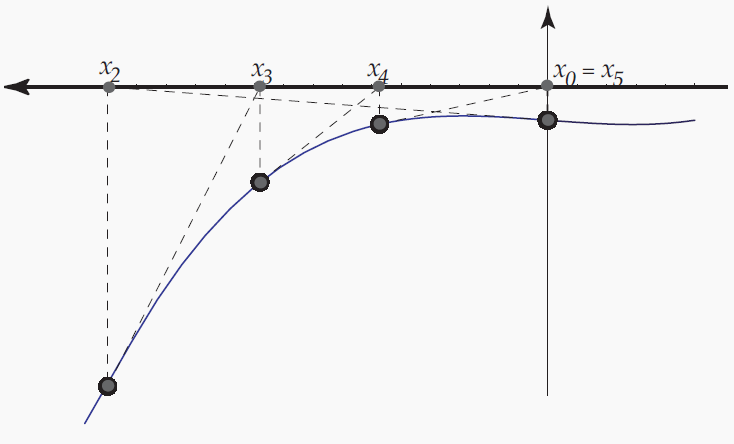
\includegraphics[scale=0.25]{images/Clase3-f2-c.PNG}}
\caption{Comportamiento del método de Newton-Raphson}
\label{fig:2}
\end{figure}

\subsection{Algoritmo del método}

La Figura \eqref{fig:2} muestra gráficamente cómo funciona la iteración: se traza la recta tangente a $f(x)$ en el punto $x_i$, y la intersección de esta recta con el eje $x$ se usa como la siguiente aproximación $x_{i+1}$.

El algoritmo puede describirse así:

\begin{enumerate}
    \item Elegir un valor inicial $x_0$ como estimación de la raíz.
    \item Calcular $\Delta x = -\dfrac{f(x)}{f'(x)}$.
    \item Actualizar $x \leftarrow x + \Delta x$.
    \item Repetir los pasos 2 y 3 hasta que $|\Delta x| < \varepsilon$ (criterio de convergencia).
\end{enumerate}

{\bf Nota:} Aunque el método es rápido si se inicia cerca de la raíz, puede fallar si la derivada se anula o si se está lejos de la solución. Por eso, a veces se combina con métodos cerrados como la bisección.

\subsection{Versión segura del método}

Una alternativa práctica es usar una versión "híbrida" que combina Newton-Raphson con bisección. Se parte de un intervalo $(a, b)$ que encierra la raíz, se inicia con el punto medio, y si una iteración de Newton-Raphson sale del intervalo, se sustituye por una iteración de bisección.

El siguiente archivo implementa esta versión:

\lstinputlisting{codes/newtonRaphson_segura.m}

\begin{ejemplo}
Encuentre la menor raíz positiva de
\[
f(x) = x^4 - 6.4x^3 + 6.45x^2 + 20.538x - 31.752
\]
\end{ejemplo}

\begin{center}
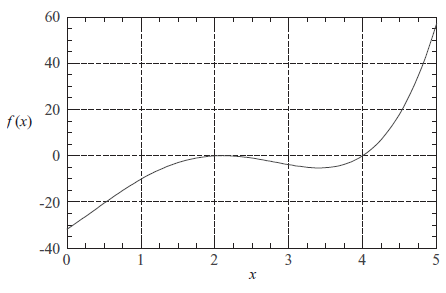
\includegraphics[scale=.5]{images/Clase3-f3.PNG}
\end{center}

Al observar el gráfico, parece que hay una raíz doble cerca de $x = 2$. La bisección no funcionaría bien en este caso, ya que la función no cambia de signo en una raíz múltiple. Sin embargo, el método de Newton-Raphson estándar sí puede aplicarse.

El siguiente programa muestra cómo usar este método para encontrar la raíz:

\lstinputlisting{codes/newton_simple.m}

Las funciones utilizadas en este ejemplo son:

\lstinputlisting{codes/fej3_1.m}
\lstinputlisting{codes/dfej3_1.m}

Y el resultado se obtiene mediante:

\lstinputlisting{codes/diary2.m}

\subsection{Raíces múltiples y convergencia modificada}

Cuando una función tiene una raíz múltiple, el método de Newton-Raphson ya no tiene convergencia cuadrática, sino {\bf lineal}. Esto explica por qué se requieren más iteraciones en el ejemplo anterior.

Para mejorar la convergencia en estos casos, se puede modificar la fórmula original del método así:
\begin{align}
x_{i+1} = x_i - m\frac{f(x_i)}{f'(x_i)} \label{eq:9}
\end{align}
donde $m$ es la multiplicidad conocida de la raíz (en el ejemplo anterior, $m = 2$). Esta modificación permite recuperar la convergencia rápida esperada.

\section{Sistema de Ecuaciones No Lineales}

Hasta ahora, hemos trabajado con funciones de una sola variable, es decir, con ecuaciones de la forma $f(x) = 0$. Sin embargo, muchos problemas reales requieren resolver sistemas de ecuaciones no lineales con varias variables. Este tipo de problemas puede expresarse como:
\[
f(x) = 0
\]
donde $f(x)$ es un vector de funciones y $x$ es un vector de variables. En notación escalar, esto equivale a:
\begin{align*}
f_1(x_1,x_2,\ldots,x_n)&=0\\
f_2(x_1,x_2,\ldots,x_n)&=0\\
&\vdots\\
f_n(x_1,x_2,\ldots,x_n)&=0
\end{align*}

Resolver este tipo de sistemas es más complejo que el caso de una sola variable. Uno de los principales desafíos es que no existe un método sencillo para asegurar que la solución esté contenida dentro de un intervalo determinado. Por lo tanto, es fundamental partir de una buena estimación inicial, la cual muchas veces proviene del análisis físico del problema.

Uno de los métodos más utilizados para resolver sistemas de ecuaciones no lineales es el {\bf método de Newton-Raphson}, ya que es relativamente fácil de implementar y converge rápidamente si se parte de una buena estimación inicial.

\subsection{El método de Newton-Raphson para sistemas}

Para extender el método de Newton-Raphson al caso de varias variables, utilizamos una expansión de Taylor de primer orden para cada función $f_i$ alrededor de un punto $x$:
\begin{align}
f_i(x + \Delta x) = f_i(x) + \sum_{j=1}^n \frac{\partial f_i}{\partial x_j} \Delta x_j + O(\Delta x^2) \label{eq:11}
\end{align}

Descartando los términos de segundo orden, esta expresión se puede escribir de manera matricial como:
\[
f(x + \Delta x) = f(x) + J(x)\Delta x
\]
donde $J(x)$ es la matriz Jacobiana, cuyos elementos son:
\[
J_{ij} = \frac{\partial f_i}{\partial x_j}
\]

Esta matriz contiene las derivadas parciales de todas las funciones con respecto a todas las variables, y representa la generalización de la derivada en el caso multivariable.

Ahora, si asumimos que $x$ es la estimación actual del vector solución, buscamos una corrección $\Delta x$ tal que:
\[
f(x + \Delta x) = 0
\]
Sustituyendo en la expansión anterior, obtenemos:
\[
J(x)\Delta x = -f(x)
\]

Este sistema de ecuaciones lineales se puede resolver para encontrar $\Delta x$, y luego se actualiza el valor de $x$:
\[
x \leftarrow x + \Delta x
\]

\subsection*{Pasos del algoritmo de Newton-Raphson para sistemas}

\begin{enumerate}
    \item Estimar un valor inicial para el vector $x$.
    \item Evaluar $f(x)$.
    \item Calcular la matriz Jacobiana $J(x)$.
    \item Resolver el sistema lineal $J(x)\Delta x = -f(x)$.
    \item Actualizar: $x \leftarrow x + \Delta x$.
    \item Repetir desde el paso 2 hasta que $||\Delta x||$ sea menor que la tolerancia.
\end{enumerate}

\subsection*{Implementación}

En el siguiente código, se implementa el método de Newton-Raphson para sistemas de ecuaciones. La función requiere que el usuario proporcione una función que evalúe el vector $f(x)$. La matriz Jacobiana se aproxima por diferencias finitas.

\lstinputlisting{codes/newtonRaphson_sistema.m}

\lstinputlisting{codes/jacobian.m}

{\bf Nota:} La matriz Jacobiana se vuelve a calcular en cada iteración. Esto puede representar un alto costo computacional si el número de variables $n$ es grande o si $f(x)$ es costoso de evaluar. Si se está cerca de la solución, es posible fijar $J(x)$ y no recalcularla en cada paso para ahorrar tiempo.

\begin{ejemplo}
Encuentre una solución del siguiente sistema:
\[
\left\lbrace
\begin{array}{l}
\sin x + y^2 + \ln z - 7 = 0\\
3x + 2^y - z^3 + 1 = 0\\
x + y + z - 5 = 0
\end{array}
\right.
\]
usando el método {\tt newtonRaphson\_sistema}, iniciando en el punto $[1, 1, 1]$.
\end{ejemplo}

Si denotamos $x = x_1$, $y = x_2$ y $z = x_3$, la función que define el sistema se implementa en:

\lstinputlisting{codes/fej4_1.m}

Para resolver el sistema, se ejecuta: \texttt{newtonRaphson\_sistema(@fej4\_1, [1; 1; 1])}.

La solución obtenida es:
\(
x = 0.5991, \quad y = 2.3959, \quad z = 2.0050
\).

\section{Problemas Propuestos}

\begin{multicols}{2}


{\problem 
\begin{itemize}
\item[a)] Aplique el método de Newton-Raphson a la función $f(x) = \tanh(x^2 - 9)$ con $x_0 = 3.2$. Realice al menos cuatro iteraciones.
\item[b)] ¿Converge el método a la raíz real? Apoye su análisis con una gráfica.
\end{itemize}}

{\problem La función $f(x) = x^3 - 2x^2 - 4x + 8$ tiene una raíz doble en $x = 2$. Resuélvala con:
\begin{itemize}
\item[a)] Newton-Raphson estándar
\item[b)] Newton-Raphson modificado
\end{itemize}
Compare la velocidad de convergencia usando $x_0 = 1.2$.}

{\problem Resuelva el siguiente sistema por:
\begin{itemize}
\item[a)] Iteración de punto fijo
\item[b)] Newton-Raphson
\end{itemize}
\[
\left\{
\begin{array}{rcl}
y &=& -x^2 + x + 0.75 \\
y + 5xy &=& x^2
\end{array}
\right.
\]
Use $x = y = 1.2$ como valor inicial. Analice los resultados.}

{\problem\label{p:1} Encuentre las raíces del siguiente sistema:
\[
\left\{
\begin{array}{rcl}
(x - 4)^2 + (y - 4)^2 &=& 5 \\
x^2 + y^2 &=& 16
\end{array}
\right.
\]
Estime gráficamente los valores iniciales y refine la solución con Newton-Raphson.}

{\problem Repita el problema (\ref{p:1}) con el sistema:
\[
\left\{
\begin{array}{rcl}
y &=& x^2 + 1 \\
y &=& 2\cos x
\end{array}
\right.
\]
Determine la raíz positiva.}

{\problem\label{p:2} El balance de masa de un contaminante en un lago bien mezclado se expresa como:
\[
V \frac{dc}{dt} = W - Qc - kV\sqrt{c}
\]
Dado:
\(
V = 1 \times 10^6 \, \text{m}^3,\quad Q = 1 \times 10^5 \, \text{m}^3/\text{año},\quad W = 1 \times 10^6 \, \text{g}/\text{año},\quad k = 0.25 \, \text{m}^{0.5}/\text{año}
\). 
Para el problema, se puede escribir la ecuación como:
\[
c = \left( \frac{W - Qc}{kV} \right)^2 \quad \text{o bien} \quad c = \frac{W - kV\sqrt{c}}{Q}
\]
De las dos formas, solo una converge para $2 < c < 6$. Determine cuál y explique por qué.}

{\problem Desarrolle un programa amigable para el usuario que implemente el método de Newton-Raphson.}

{\problem Desarrolle un programa amigable para el método de Newton-Raphson aplicado a sistemas de ecuaciones.}

\end{multicols}

\end{document}